\documentclass[aspectratio=169,10pt]{beamer}
\usetheme{Madrid}
\usecolortheme{seahorse}
\usepackage{booktabs}
\usepackage{graphicx}
\usepackage{amsmath}
\setbeamertemplate{navigation symbols}{}
\setbeamertemplate{caption}{\raggedright\insertcaption\par}
\graphicspath{{./}}
\title[DIY PCA pillars]{Heat-Risk Viewer: PCA Pillar Analysis}
\subtitle{Method as implemented, with per-component loadings}
\author{San Diego County Heat-Risk Viewer}
\date{\today}

\begin{document}

\begin{frame}[plain]
  \titlepage
\end{frame}

\begin{frame}{How each pillar score is built}
  Three pillars --- \textbf{Heat Exposure}, \textbf{Population Sensitivity},
  \textbf{Adaptive Capacity} --- each reduced to one tract-level score by PCA on the
  variables the user enables. Computed client-side (Jacobi eigendecomposition).
  \begin{enumerate}\setlength\itemsep{2pt}
    \item \textbf{Standardize}: z-score each variable across all 735 tracts.
    \item \textbf{Polarity-align}: flip variables so higher always means higher risk.
    \item \textbf{Decompose}: eigendecomposition of the correlation matrix.
    \item \textbf{Retain}: keep PCs with eigenvalue $> 1$ (Kaiser rule), at least 1.
    \item \textbf{Composite}: variance-weighted sum of retained PC scores
          $\;w_i=\sum_{k\le n_{\mathrm{ret}}} \dfrac{\lambda_k}{\sum\lambda}\, s_{ik}$,
          sign-aligned to a reference variable.
    \item \textbf{Rank}: percentile-rank $w$ across the county (0--100).
  \end{enumerate}
  \footnotesize Composite risk = mean of the three pillar percentile scores
  (Adaptive Capacity inverted). Reference variables: mean $T_{max}$ (exposure),
  high blood pressure (sensitivity), income (adaptive).
\end{frame}

\begin{frame}{Heat Exposure --- variance structure}
  \centering
  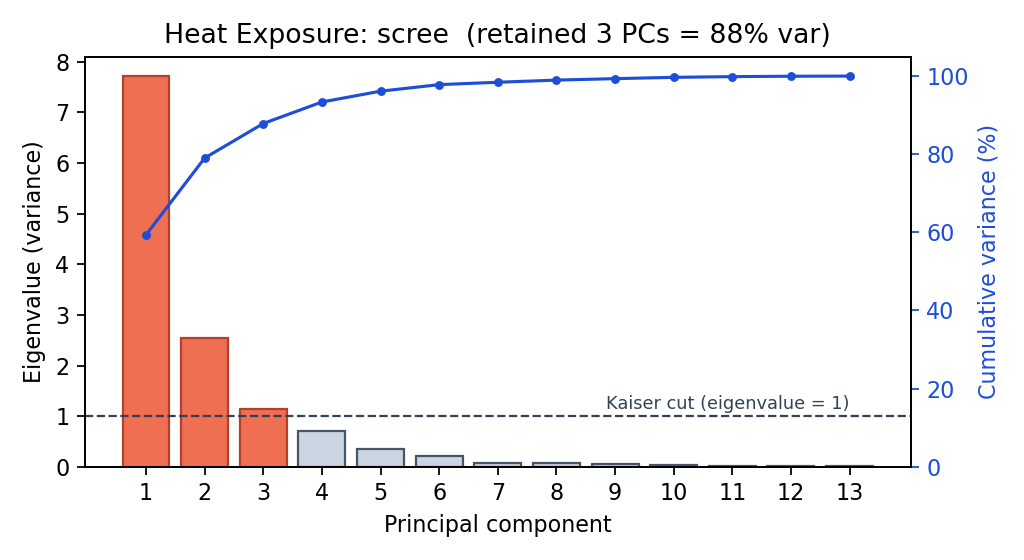
\includegraphics[width=0.92\linewidth]{fig/scree_exposure.png}\\[2pt]
  \footnotesize 13 variables enabled. Eigenvalues: 7.72, 2.55, 1.15, 0.72, 0.36, 0.22, 0.08, 0.07, \ldots.\\
  Retained 3 PCs (eigenvalue $>1$), spanning 88\% of total variance.
\end{frame}

\begin{frame}{Heat Exposure --- loadings on each PC}
  \centering
  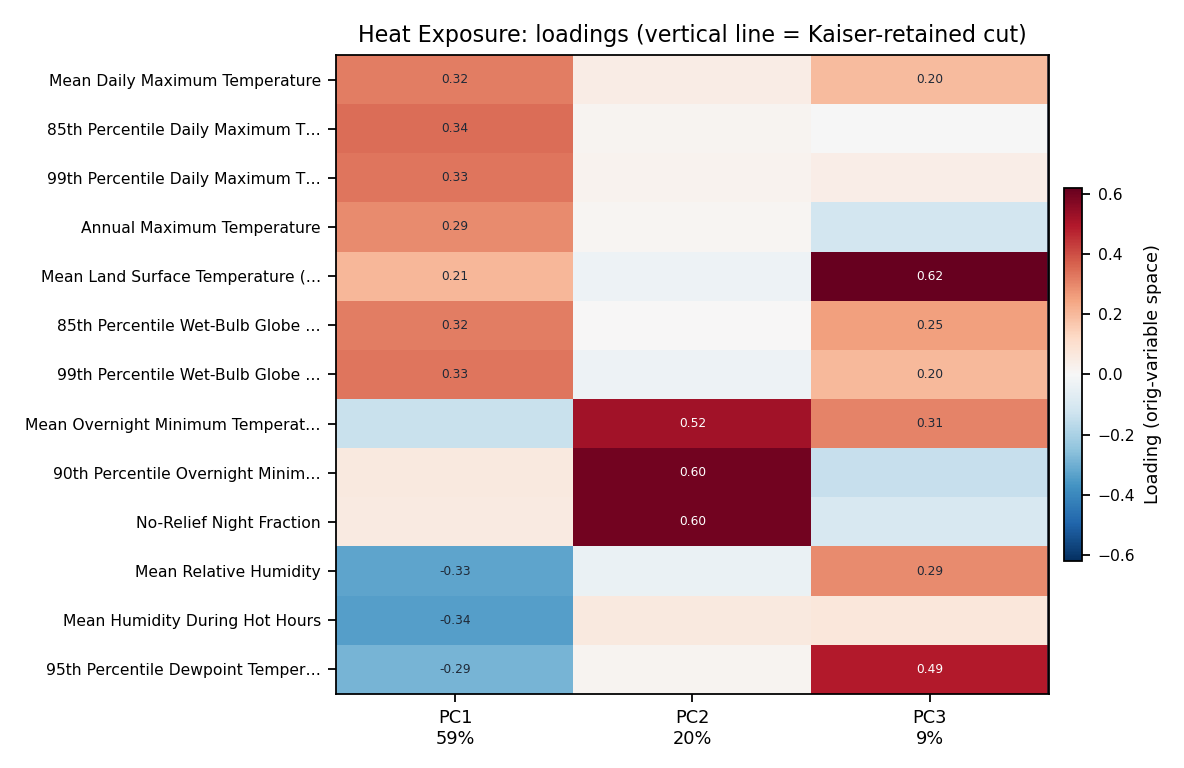
\includegraphics[height=0.86\textheight]{fig/load_exposure.png}
\end{frame}

\begin{frame}{Heat Exposure --- strongest loadings per component}
  \centering\footnotesize
  \begin{tabular}{lll}
    \toprule
    \textbf{PC1} (59\%) & \textbf{PC2} (20\%) & \textbf{PC3} (9\%) \\ \midrule
85th Percentile Daily… (+0.34) & No-Relief Night Fract… (+0.60) & Mean Land Surface Tem… (+0.62) \\
Mean Humidity During … (-0.34) & 90th Percentile Overn… (+0.60) & 95th Percentile Dewpo… (+0.49) \\
99th Percentile Wet-B… (+0.33) & Mean Overnight Minimu… (+0.52) & Mean Overnight Minimu… (+0.31) \\
99th Percentile Daily… (+0.33) & Mean Humidity During … (+0.06) & Mean Relative Humidity (+0.29) \\
Mean Relative Humidity (-0.33) & Mean Daily Maximum Te… (+0.05) & 85th Percentile Wet-B… (+0.25) \\
85th Percentile Wet-B… (+0.32) & Mean Relative Humidity (-0.04) & 99th Percentile Wet-B… (+0.20) \\
    \bottomrule
  \end{tabular}\\[6pt]
  \scriptsize Each cell: variable (signed loading in original-variable space).
  Positive $=$ higher value of that variable pushes the pattern toward higher risk.
\end{frame}

\begin{frame}{Population Sensitivity --- variance structure}
  \centering
  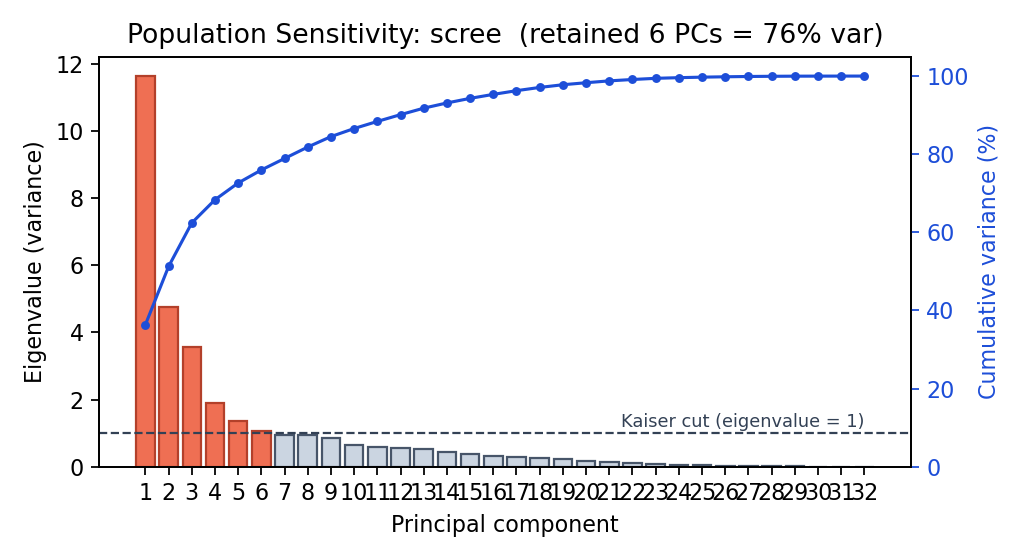
\includegraphics[width=0.92\linewidth]{fig/scree_sensitivity.png}\\[2pt]
  \footnotesize 32 variables enabled. Eigenvalues: 11.64, 4.77, 3.57, 1.90, 1.37, 1.07, 0.94, 0.94, \ldots.\\
  Retained 6 PCs (eigenvalue $>1$), spanning 76\% of total variance.
\end{frame}

\begin{frame}{Population Sensitivity --- loadings on each PC}
  \centering
  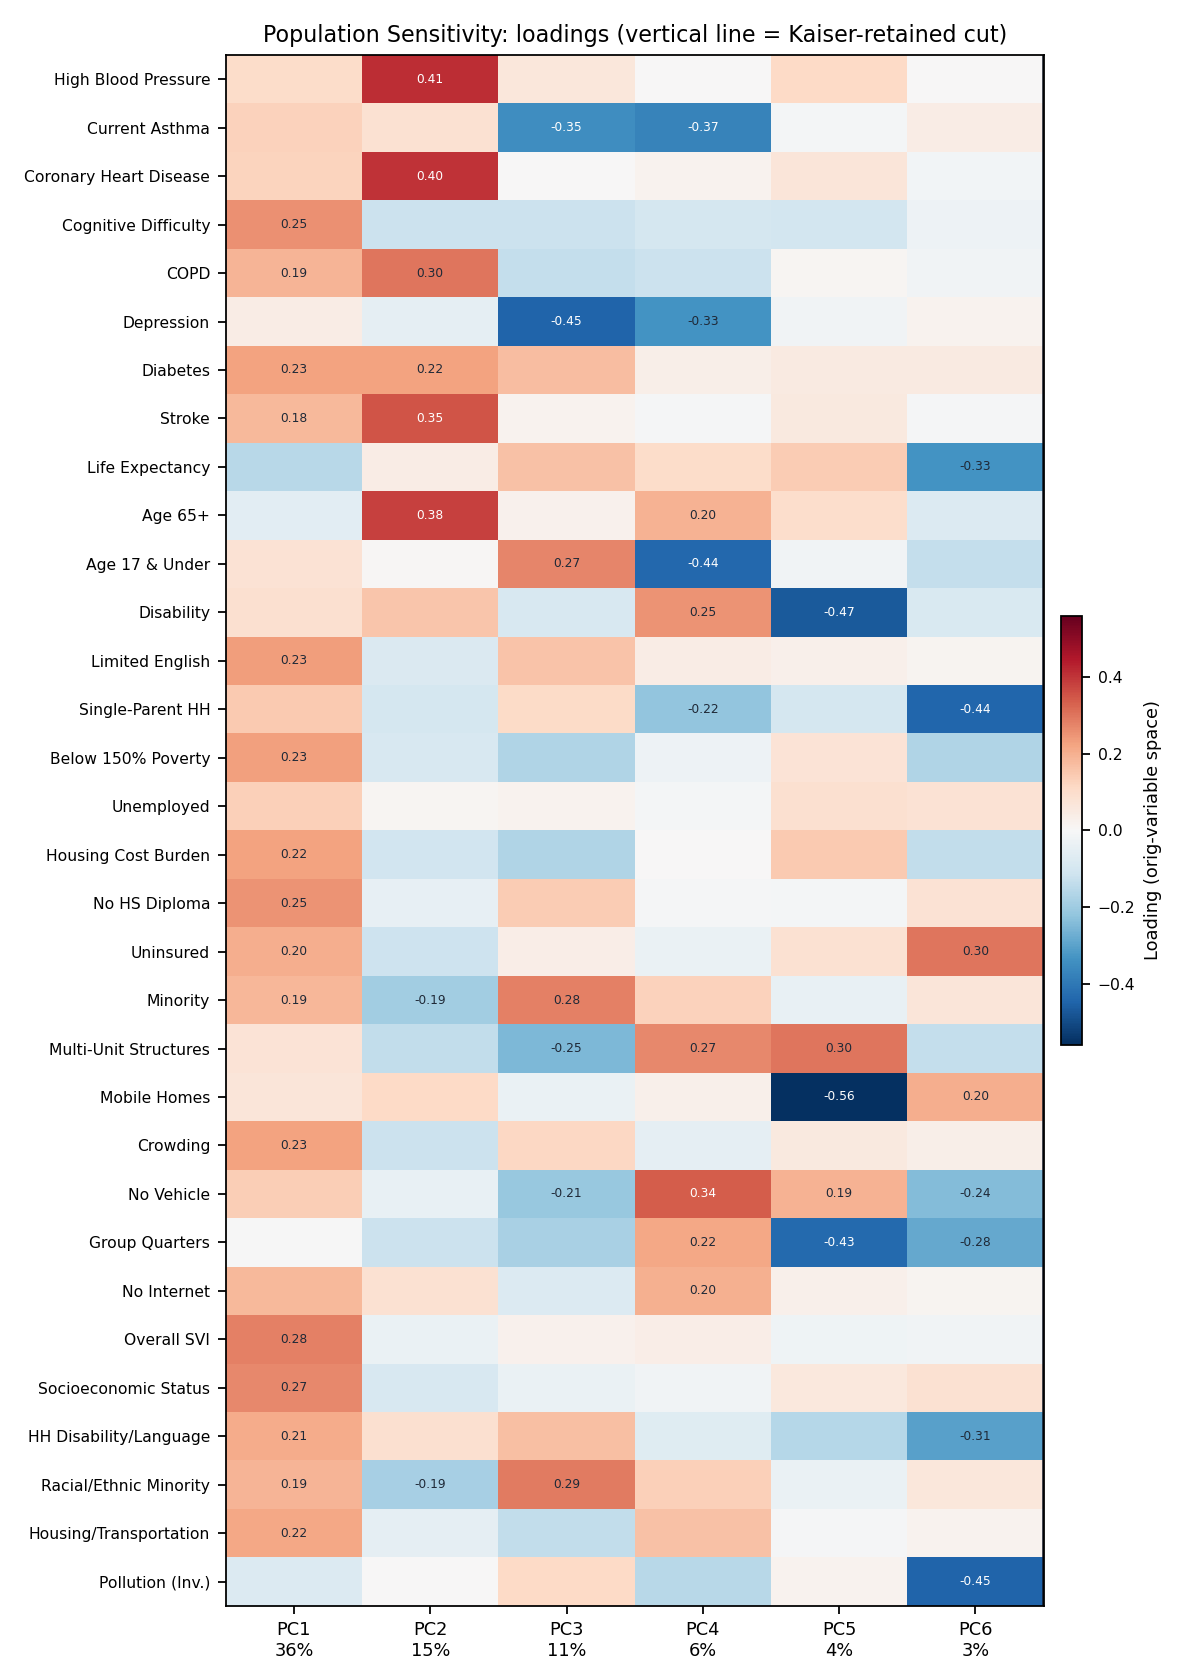
\includegraphics[height=0.86\textheight]{fig/load_sensitivity.png}
\end{frame}

\begin{frame}{Population Sensitivity --- strongest loadings per component}
  \centering\footnotesize
  \begin{tabular}{lll}
    \toprule
    \textbf{PC1} (36\%) & \textbf{PC2} (15\%) & \textbf{PC3} (11\%) \\ \midrule
Overall SVI (+0.28) & High Blood Pressure (+0.41) & Depression (-0.45) \\
Socioeconomic Status (+0.27) & Coronary Heart Disease (+0.40) & Current Asthma (-0.35) \\
Cognitive Difficulty (+0.25) & Age 65+ (+0.38) & Racial/Ethnic Minority (+0.29) \\
No HS Diploma (+0.25) & Stroke (+0.35) & Minority (+0.28) \\
Limited English (+0.23) & COPD (+0.30) & Age 17 \& Under (+0.27) \\
Below 150\% Poverty (+0.23) & Diabetes (+0.22) & Multi-Unit Structures (-0.25) \\
    \bottomrule
  \end{tabular}\\[6pt]
  \scriptsize Each cell: variable (signed loading in original-variable space).
  Positive $=$ higher value of that variable pushes the pattern toward higher risk.
\end{frame}

\begin{frame}{Adaptive Capacity --- variance structure}
  \centering
  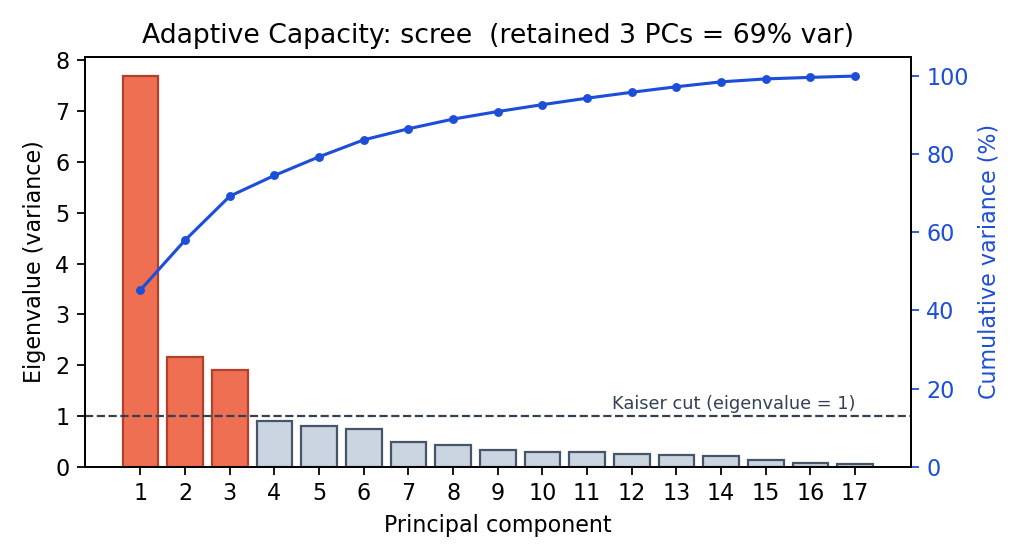
\includegraphics[width=0.92\linewidth]{fig/scree_adaptive.png}\\[2pt]
  \footnotesize 17 variables enabled. Eigenvalues: 7.69, 2.17, 1.91, 0.90, 0.81, 0.74, 0.48, 0.42, \ldots.\\
  Retained 3 PCs (eigenvalue $>1$), spanning 69\% of total variance.
\end{frame}

\begin{frame}{Adaptive Capacity --- loadings on each PC}
  \centering
  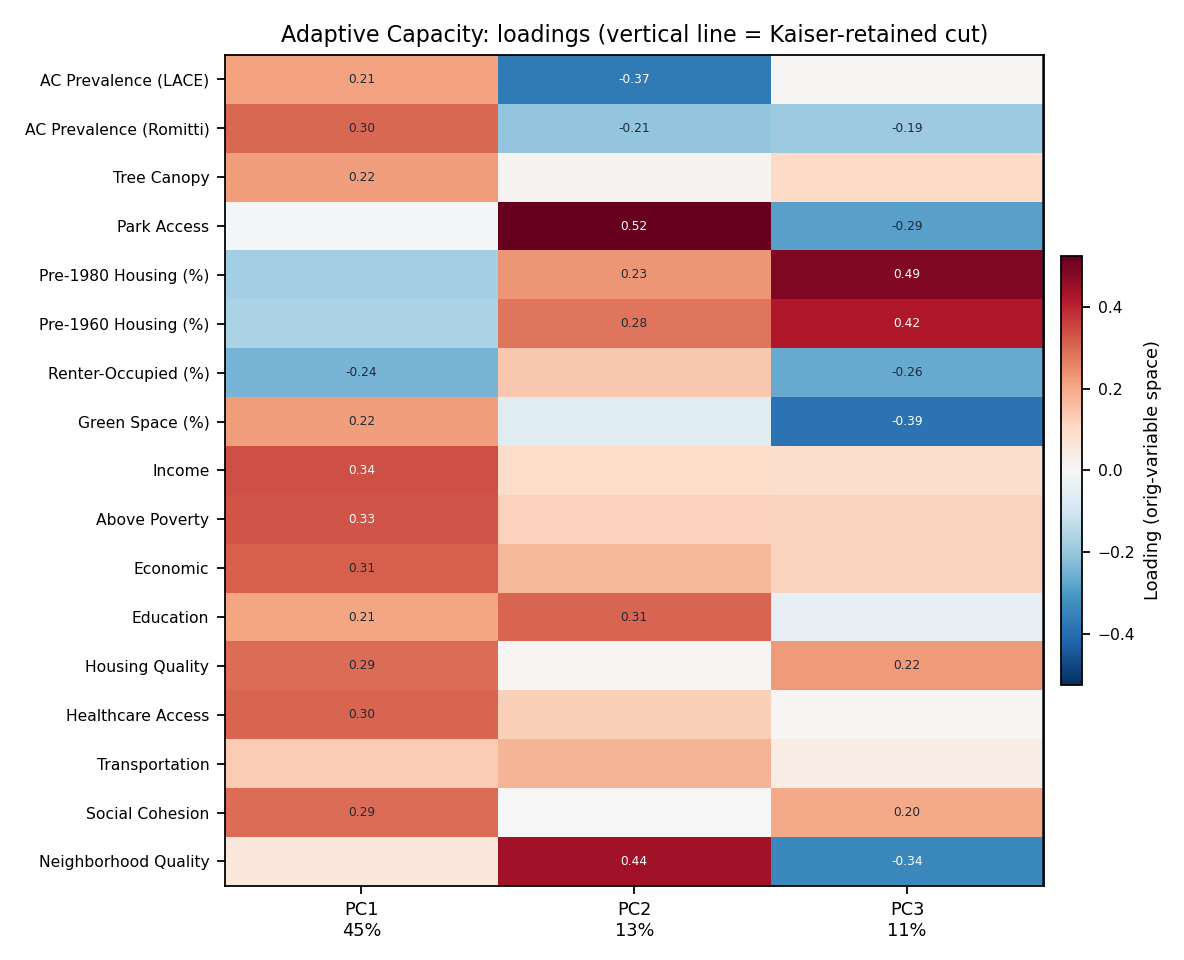
\includegraphics[height=0.86\textheight]{fig/load_adaptive.png}
\end{frame}

\begin{frame}{Adaptive Capacity --- strongest loadings per component}
  \centering\footnotesize
  \begin{tabular}{lll}
    \toprule
    \textbf{PC1} (45\%) & \textbf{PC2} (13\%) & \textbf{PC3} (11\%) \\ \midrule
Income (+0.34) & Park Access (+0.52) & Pre-1980 Housing (\%) (+0.49) \\
Above Poverty (+0.33) & Neighborhood Quality (+0.44) & Pre-1960 Housing (\%) (+0.42) \\
Economic (+0.31) & AC Prevalence (LACE) (-0.37) & Green Space (\%) (-0.39) \\
Healthcare Access (+0.30) & Education (+0.31) & Neighborhood Quality (-0.34) \\
AC Prevalence (Romitt… (+0.30) & Pre-1960 Housing (\%) (+0.28) & Park Access (-0.29) \\
Housing Quality (+0.29) & Pre-1980 Housing (\%) (+0.23) & Renter-Occupied (\%) (-0.26) \\
    \bottomrule
  \end{tabular}\\[6pt]
  \scriptsize Each cell: variable (signed loading in original-variable space).
  Positive $=$ higher value of that variable pushes the pattern toward higher risk.
\end{frame}

\begin{frame}{What the composite actually is}
  The pillar score collapses the retained PCs back to one number --- a linear
  weighted combination of the inputs. Because a PC's spread scales as
  $\sqrt{\lambda}$ \emph{and} it is weighted by $\lambda$, the contribution of
  each component scales as $\lambda^{1.5}$: PC1 dominates.
  \begin{center}\small
  \begin{tabular}{lcccc}
    \toprule
    Pillar & PC1 var & Retained & \multicolumn{2}{c}{Spearman of score vs.} \\
           &         &          & equal-wt avg & PC1 alone \\
    \midrule
    Heat Exposure & 59\% & 3 (88\%) & 0.68 & 0.99 \\
Population Sensitivity & 36\% & 6 (76\%) & 0.87 & 0.93 \\
Adaptive Capacity & 45\% & 3 (69\%) & 0.96 & 0.98 \\
    \bottomrule
  \end{tabular}
  \end{center}
  \footnotesize
  PCA's value here is \textbf{redundancy-aware weighting} ($\approx$ PC1): the more
  correlated the inputs (e.g.\ exposure's many temperature measures), the more the
  score departs from a plain average. The retained-count / cumulative-variance
  figures describe the PC \emph{set}, not how much the final score uses --- that is
  effectively PC1.
\end{frame}
\end{document}
